\chapter{Hardware}

%TODO choix composants (IMU, GPS)? position carte?

\section{Architecture}

\begin{figure}[H]
    \centering
    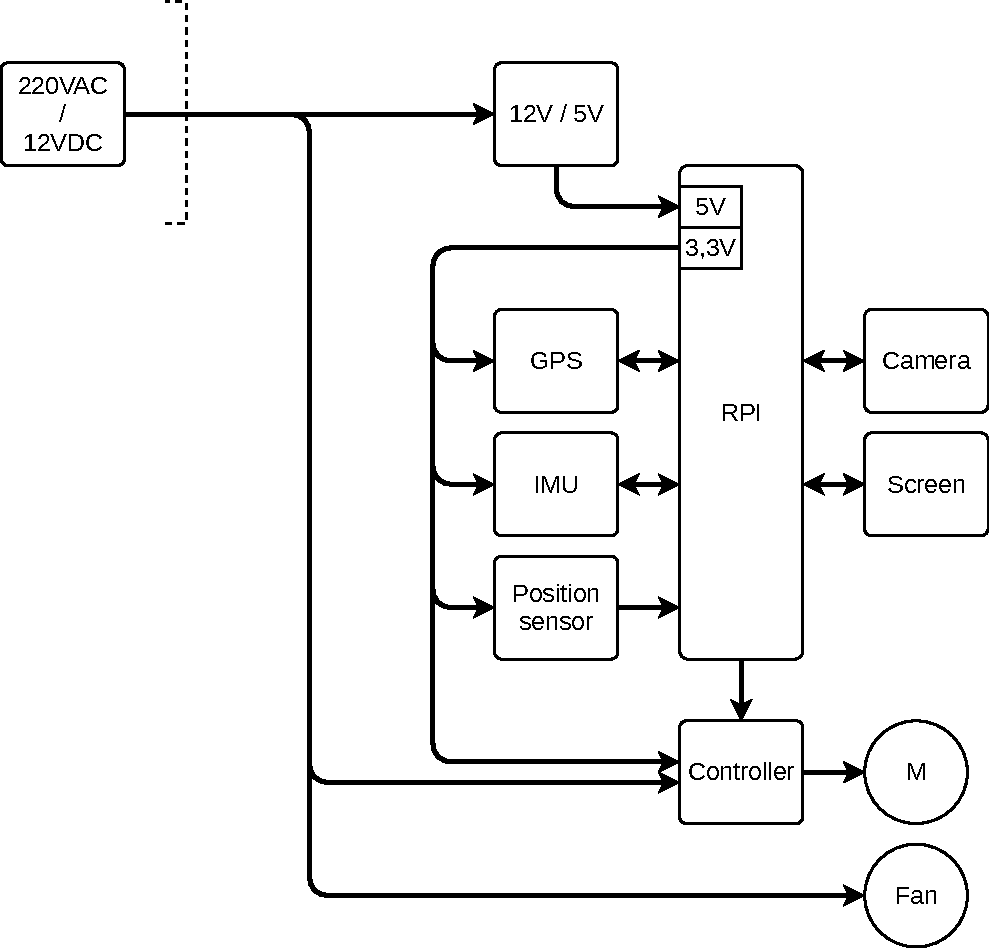
\includegraphics[width=0.7\linewidth]{\figures/sch_hardware3.pdf}
    \decoRule
    \caption[
    Schéma structurel de premier niveau du télescope]{
    Schéma structurel de premier niveau du télescope}
    \label{fig:Schéma structurel de premier niveau du télescope}
    \end{figure}

\vspace{1cm}

La première question de l'étude structurelle du télescope est celle de l'alimentation.

Le télescope sera raccordé au secteur par un module externe $220VAC / 12VDC$. Ensuite les moteurs seront alimentés en $12V$ via leurs contrôleurs respectifs et la Raspberry-Pi sera alimentée en 5V. Un convertisseur $12V / 5V$ est donc a ajouter.

Le télescope est également doté d'un ventilateur situé sous le miroir primaire et servant à le maintenir à température constante. Celui-ci sera alimenté en $12V$.

\vspace{1cm}

Tous les autres éléments seront alimentés en $3,3V$ par la Raspberry-Pi. Il est toutefois important de s'assurer que la consommation maximale en courant de ces élément ne dépasse pas ce que peut fournir la Raspberry-Pi, à savoir $500mA$.
\begin{itemize}[label=$\bullet$]
	\item Contrôleurs des moteurs ($\times 3$)~: $8mA$
	\item GPS~: $25mA$
	\item IMU~: $3,7mA$
	\item Capteurs de position des moteurs ($\times 5$)~: $33\mu A$
	\end{itemize}

\vspace{1cm}

La consommation en courant totale des périphériques de la Raspberry-Pi est largement inférieure à $500mA$, le montage est donc réalisable sans risque de dysfonctionnement ou de dommages.

\section{Conception du circuit}

\begin{figure}[H]
    \centering
    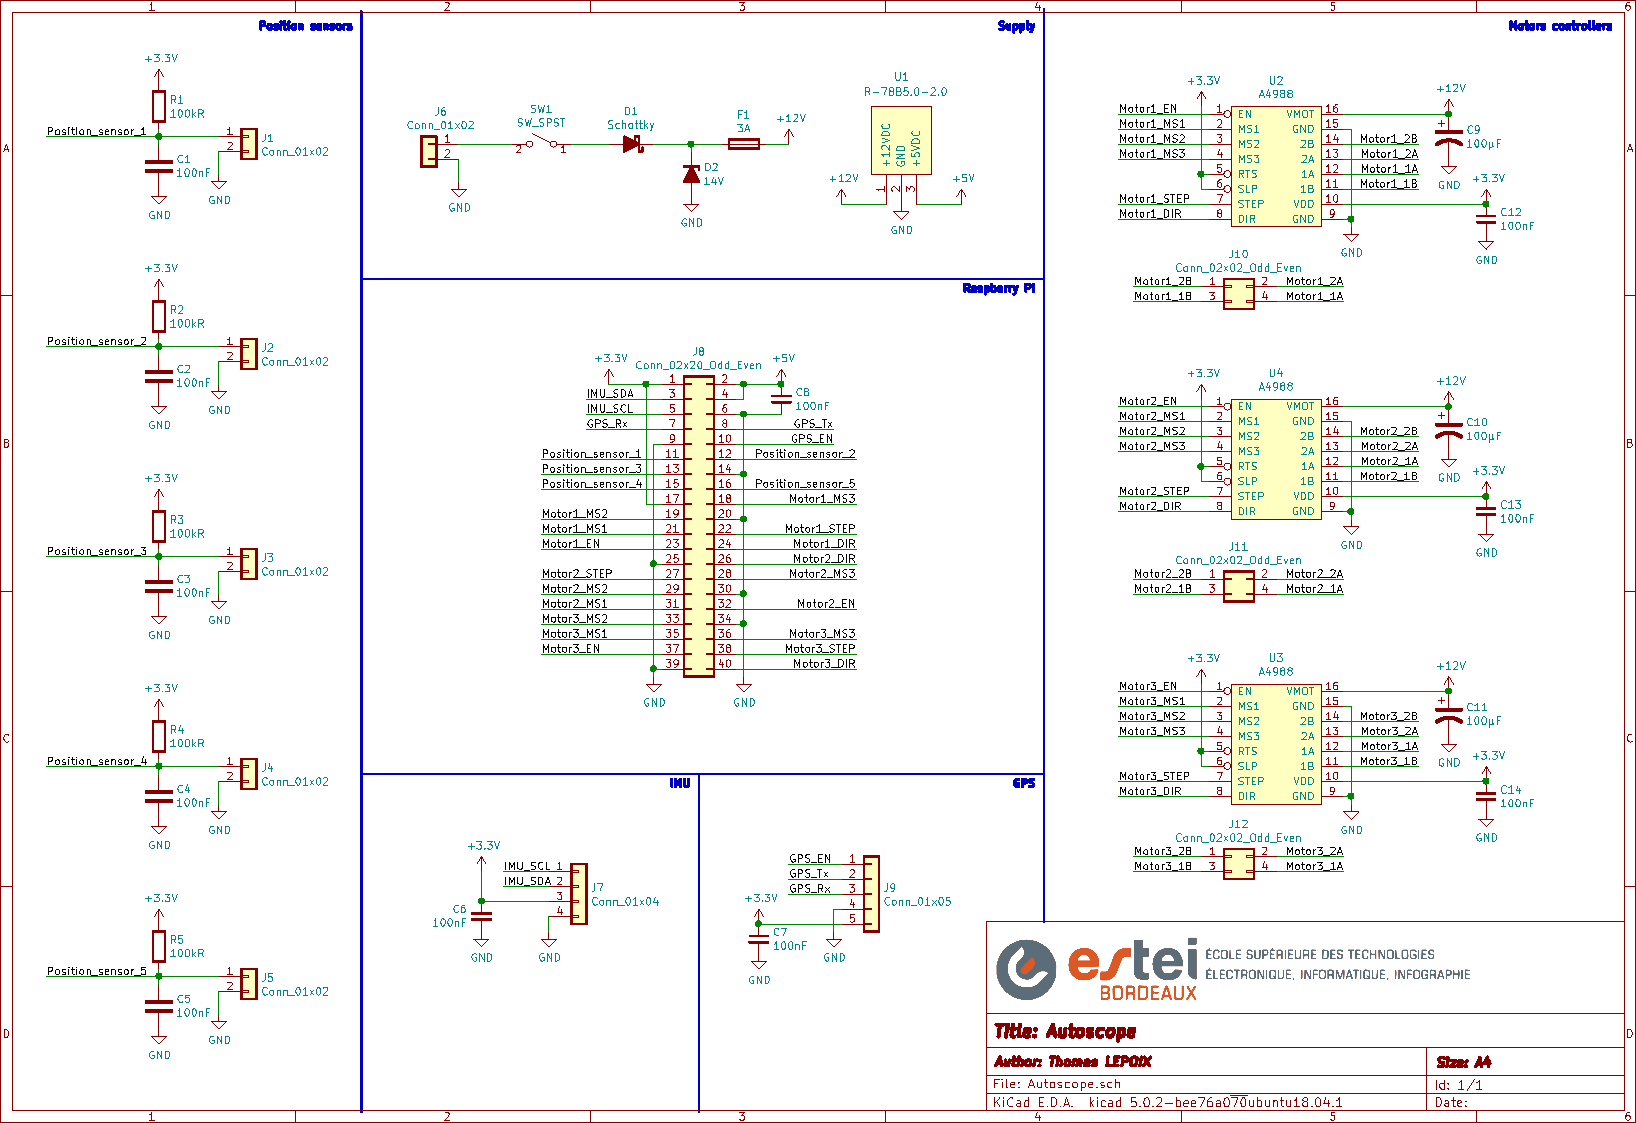
\includegraphics[width=1\linewidth]{\figures/kicad_sch2.pdf}
    \decoRule
    \caption[
    Schéma structurel de la carte du télescope]{
    Schéma structurel de la carte du télescope}
    \label{fig:Schéma structurel de la carte du télescope}
    \end{figure}

\vspace{1cm}

Ce schéma ne présente pas de subtilité particulière, la plupart des composants étant des connecteurs.

\vspace{1cm}

L'alimentation est composée de~:
\begin{itemize}[label=$\bullet$]
	\item Un interrupteur d'allumage
	\item Une diode polarisante
	\item Une diode zener (TVS) protégeant des surtensions
	\item Un fusible protégeant des surintensités
	\item Un convertisseur DC/DC intégré
	\end{itemize}

\vspace{1cm}

L'environnement des boutons poussoirs servant de capteurs de butée aux mouvements du télescope est le suivant~:

\begin{figure}[H]
    \centering
    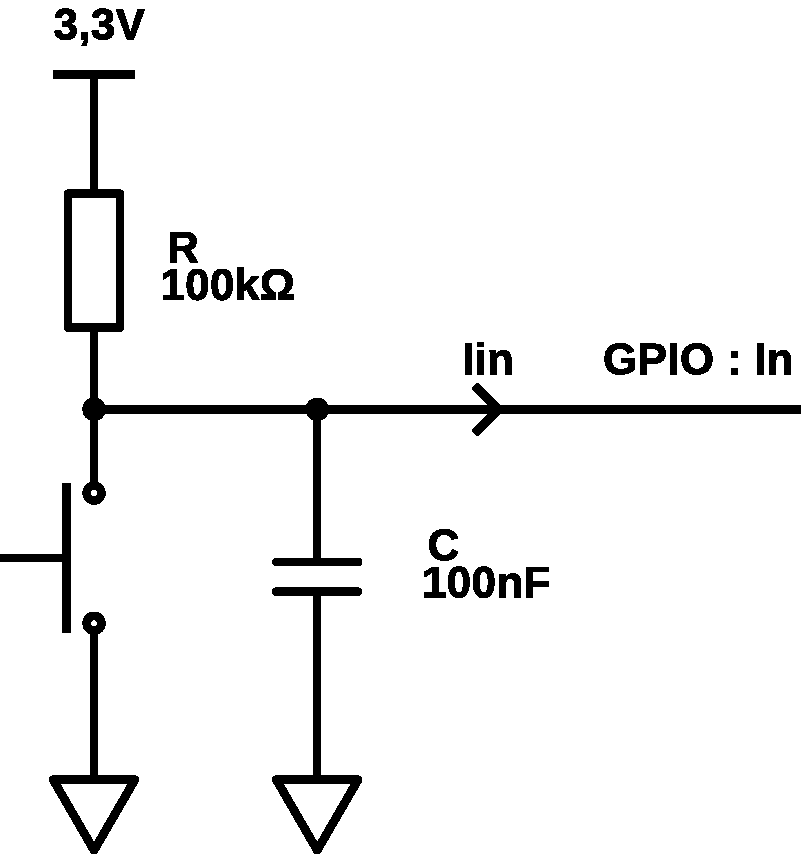
\includegraphics[width=0.3\linewidth]{\figures/sch_button.pdf}
    \decoRule
    \caption[
    Schéma de l'environnement des capteurs de butée]{
    Schéma de l'environnement des capteurs de butée}
    \label{fig:Schéma de l'environnement des capteurs de butée}
    \end{figure}

\vspace{1cm}

La valeur élevée des résistances de pullup $100k\Omega$ a pour but de réduire au maximum le courant consommé lors de l'appui, à $33\mu A$. Le courant prélevé par l'entrée GPIO de la Raspberry-Pi est de l'ordre de $0,5\mu A$.

Les condensateurs de $100nF$ permettent de filtrer les parasites générés par les rebonds propres aux boutons ainsi que les perturbations électromagnétiques.

\section{Contraintes de design}

\subsection{Contraintes électromagnétiques}

La première contrainte vient de la proximité du système électronique de deux moteurs, ceux-ci générant d'importantes perturbations électromagnétiques. Cela peut être particulièrement dérangeant pour le fonctionnement de la centrale inertielle et du GPS.

La solution la plus simple et efficace est de déporter ces deux modules le long de la structure du télescope.

%\vspace{1cm}

\subsection{Contraintes mécaniques}

Ensuite viennent les contraintes mécaniques de l'association de la carte à la Raspberry-Pi.

\vspace{1cm}

Tout d'abord, l'emplacement du connecteur et des fixations sont à prendre en compte.

\begin{figure}[H]
    \centering
    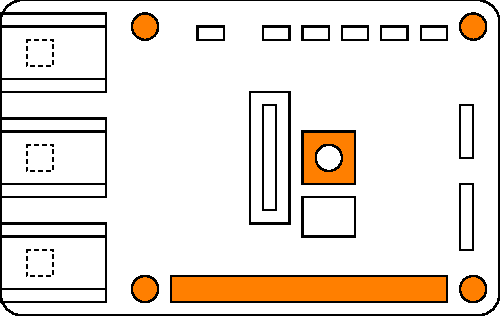
\includegraphics[width=0.5\linewidth]{\figures/sch_hard_1.pdf}
    \decoRule
    \caption[
    Schéma mécanique de la carte vue de dessus]{
    Schéma mécanique de la carte vue de dessus}
    \label{fig:Schéma mécanique de la carte vue de dessus}
    \end{figure}

\vspace{1cm}

Le connecteur d'alimentation, centré sur la carte, est un connecteur cylindrique comme ceux des ordinateurs portables. Le télescope étant amené à tourner sur lui même, ce connecteur devrait permettre le mouvement tout en empêchant le câble d'alimentation de s'emmêler ou de se détériorer.

\begin{figure}[H]
    \centering
    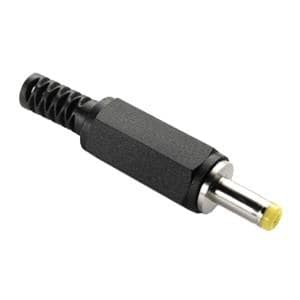
\includegraphics[height=0.3\linewidth]{\figures/photo_supply.jpg}
	\hspace{1cm}
    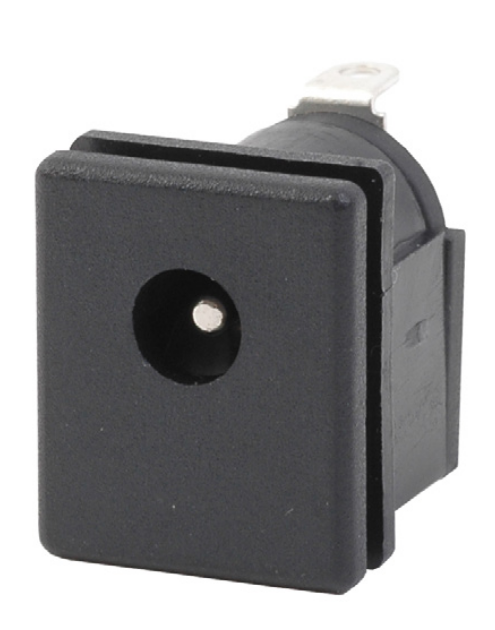
\includegraphics[height=0.3\linewidth]{\figures/photo_supply.png}
    \decoRule
    \caption[
    Connecteurs d'alimentation utilisés]{
    Connecteurs d'alimentation utilisés}
    \label{fig:Connecteurs d'alimentation utilisés}
    \end{figure}

\vspace{1cm}

Puis concernant la distance entre la carte et la Raspberry-Pi, la hauteur des plus hauts éléments de la Raspberry-Pi est à prendre en compte. Ainsi que la hauteur de certains condensateurs de la carte, ne pouvant donc être placés n'importe où.

\begin{figure}[H]
    \centering
    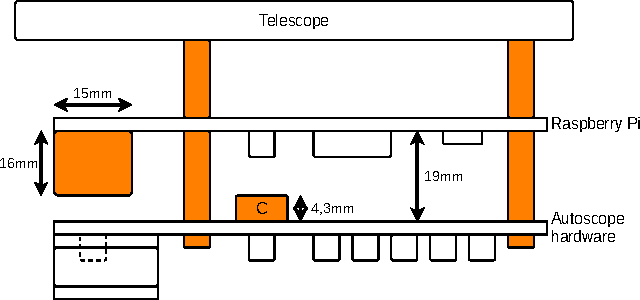
\includegraphics[height=0.23\linewidth]{\figures/sch_hard_2.pdf}
%	\hspace{1cm}
    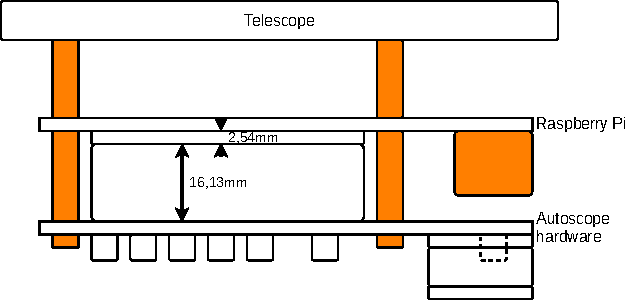
\includegraphics[height=0.23\linewidth]{\figures/sch_hard_3.pdf}
    \decoRule
    \caption[
    Schéma mécanique de la carte vue de profil]{
    Schéma mécanique de la carte vue de profil}
    \label{fig:Schéma mécanique de la carte vue de profil}
    \end{figure}

\vspace{1cm}

Il faudra de plus utiliser un connecteur particulièrement haut ($16,13mm$) pour relier la carte à la Raspberry-Pi.

\begin{figure}[H]
    \centering
    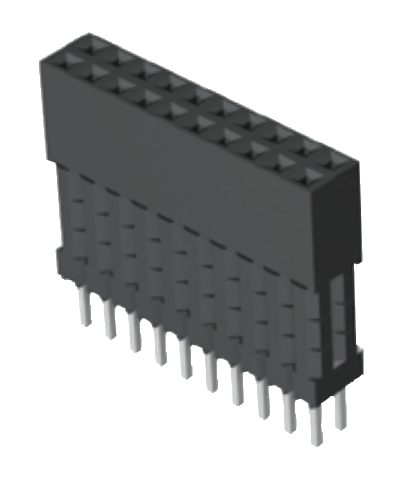
\includegraphics[width=0.3\linewidth]{\figures/photo_header.png}
    \decoRule
    \caption[
    Type de header utilisé]{
    Type de header utilisé}
    \label{fig:Type de header utilisé}
    \end{figure}

\newpage
\section{Bon de commande} %TODO prix TVS

Figurent sur le bon de commande tous les éléments faisant partie du télescope, on observe ainsi le prix de chaque partie~:
\begin{itemize}[label=$\bullet$]
	\item Éléments optiques~: $454$€
	\item Motorisation~: $64,7$€
	\item Système électronique~: $197,49$€ dont~:
	\begin{itemize}
		\item Raspberry-Pi, caméra et carte mémoire~: $61,28$€
		\item Carte électronique Autoscope~: $158,48$€
		\end{itemize}
	\end{itemize}

\vspace{1cm}

Le vert représente les composants déjà reçus, le jaune ceux commandés et le orange ceux qui seront considérés plus tard.

\begin{figure}[H]
    \centering
    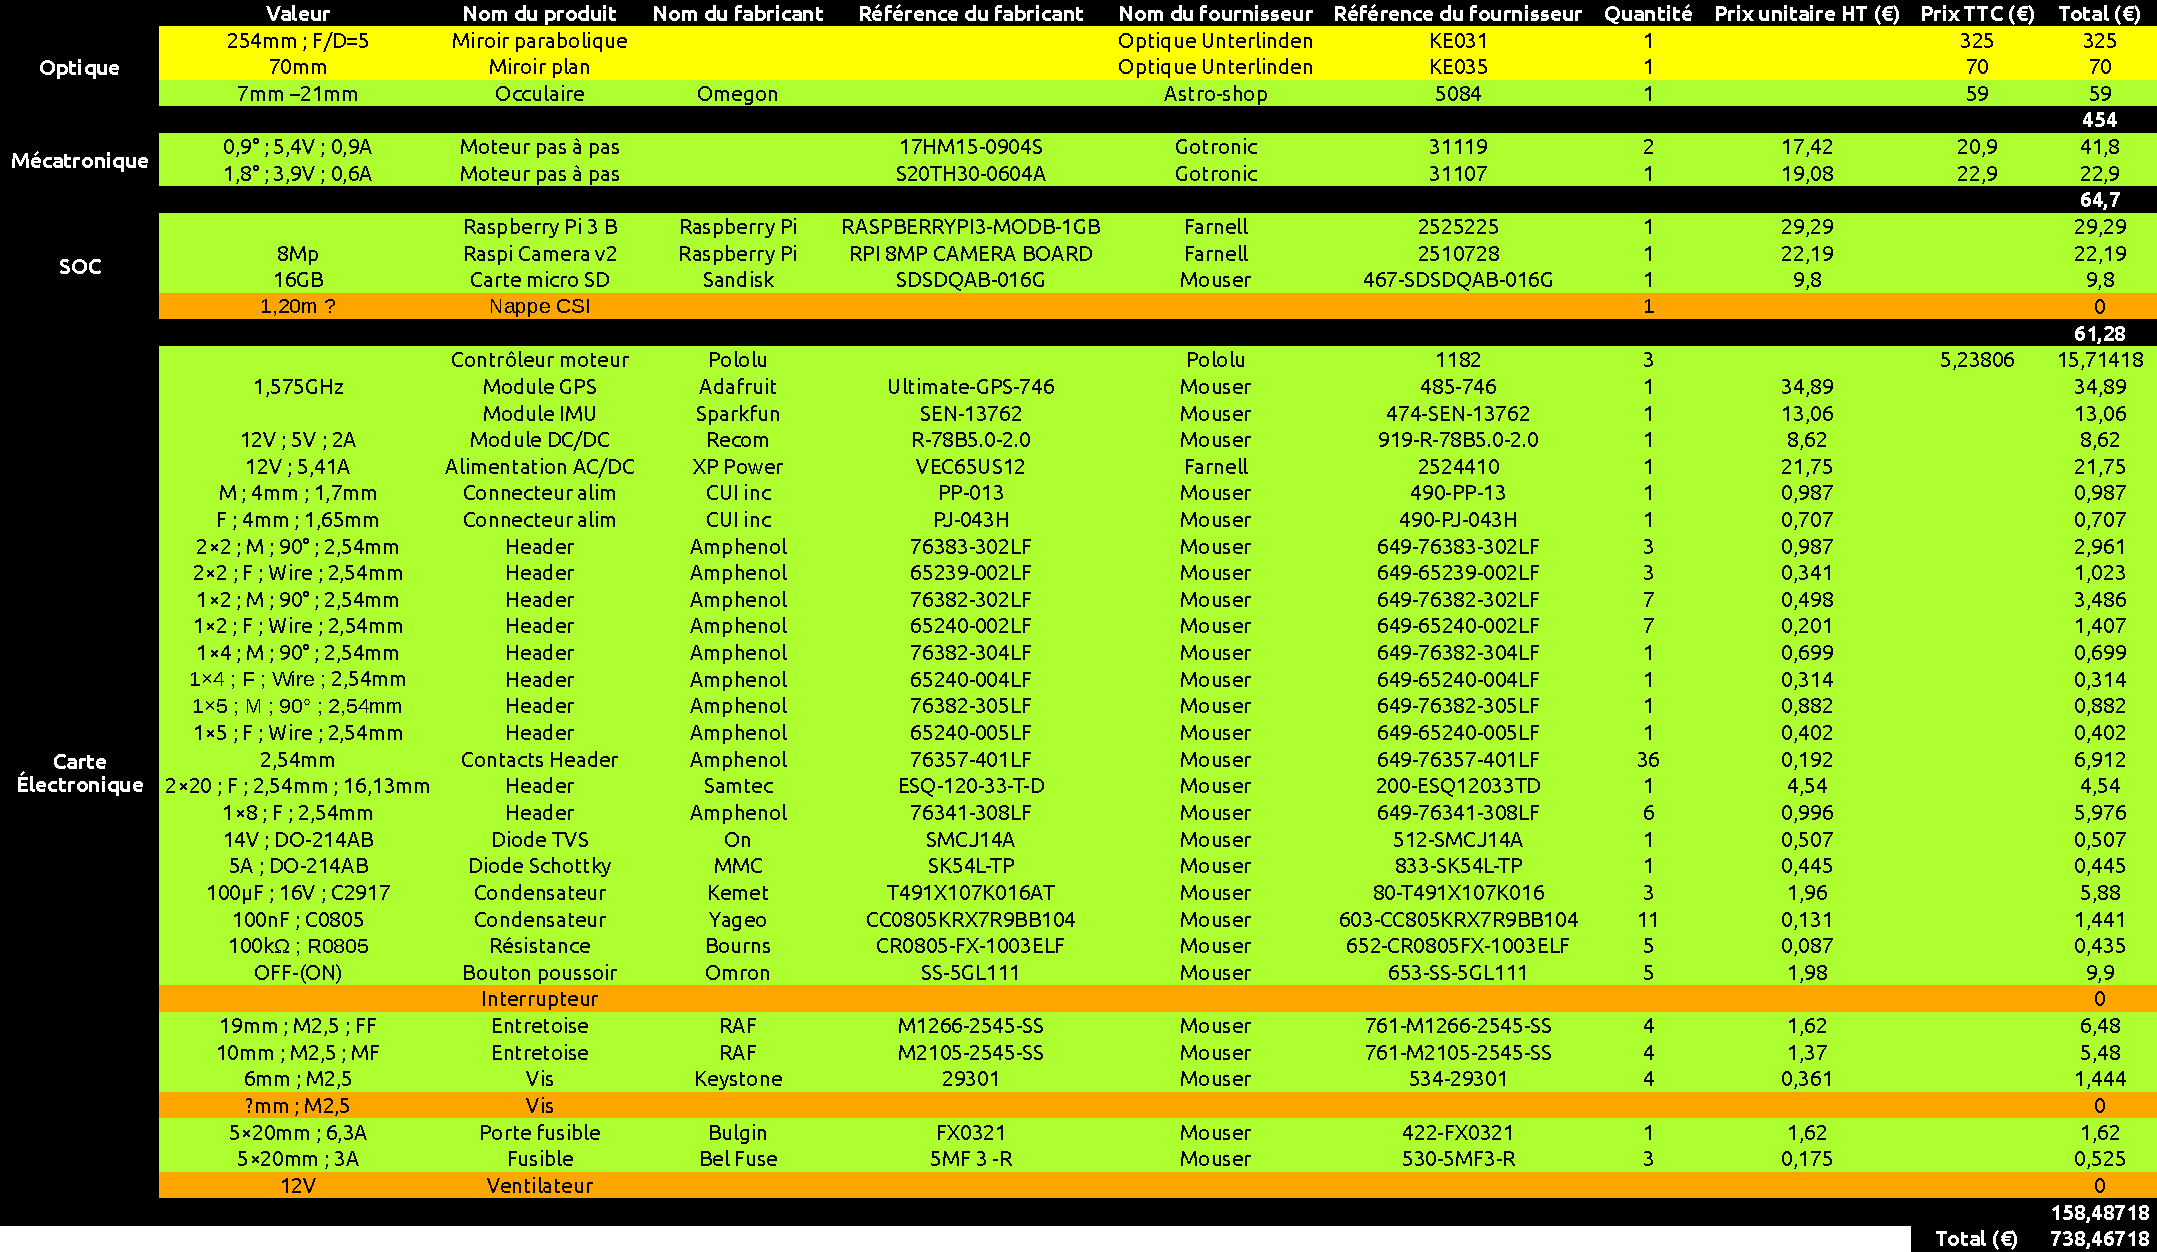
\includegraphics[width=1\linewidth]{\figures/tab_bom.pdf}
    \decoRule
    \caption[
    Bon de commande du matériel du télescope]{
    Bon de commande du matériel du télescope}
    \label{fig:Bon de commande du matériel du télescope}
    \end{figure}

\newpage
\section{Fichiers de fabrication}

\begin{figure}[H]
    \centering
    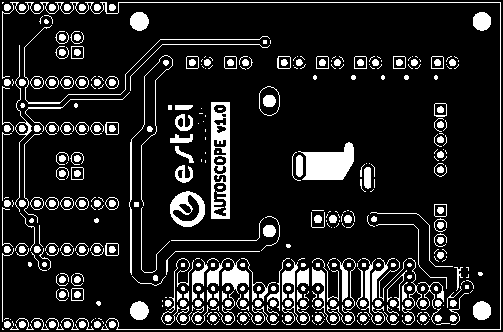
\includegraphics[width=0.49\linewidth]{\figures/kicad_f2.pdf}
    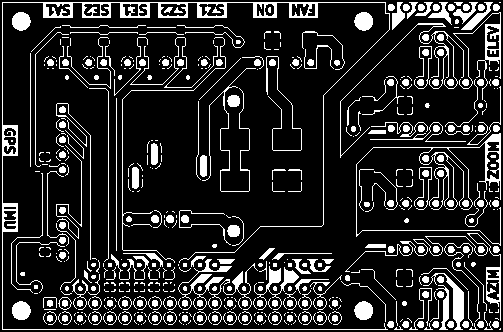
\includegraphics[width=0.49\linewidth]{\figures/kicad_b2.pdf}
    \decoRule
    \caption[
    Faces supérieure et inférieure du typon de la carte\\(respectivement vues de dessus et de dessous)]{
    Faces supérieure et inférieure du typon de la carte\\(respectivement vues de dessus et de dessous)}
    \label{fig:Faces supérieure et inférieure du typon de la carte (respectivement vues de dessus et de dessous)}
    \end{figure}

\begin{figure}[H]
    \centering
    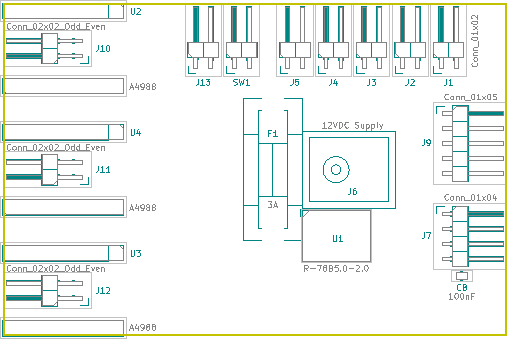
\includegraphics[width=0.49\linewidth]{\figures/kicad_cf.pdf}
    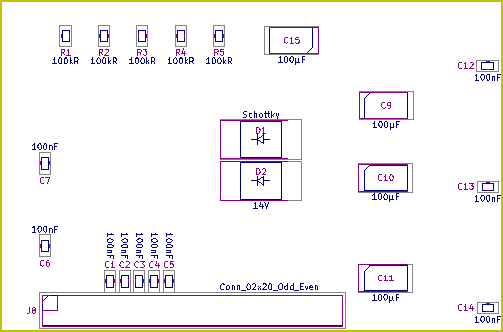
\includegraphics[width=0.49\linewidth]{\figures/kicad_cb.pdf}
    \decoRule
    \caption[
    Faces supérieure et inférieure de l'implantation des composants\\(respectivement vues de dessus et de dessous)]{
    Faces supérieure et inférieure de l'implantation des composants\\(respectivement vues de dessus et de dessous)}
    \label{fig:Faces supérieure et inférieure de l'implantation des composants (respectivement vues de dessus et de dessous)}
    \end{figure}

\section{Modélisation 3D}

\begin{figure}[H]
    \centering
    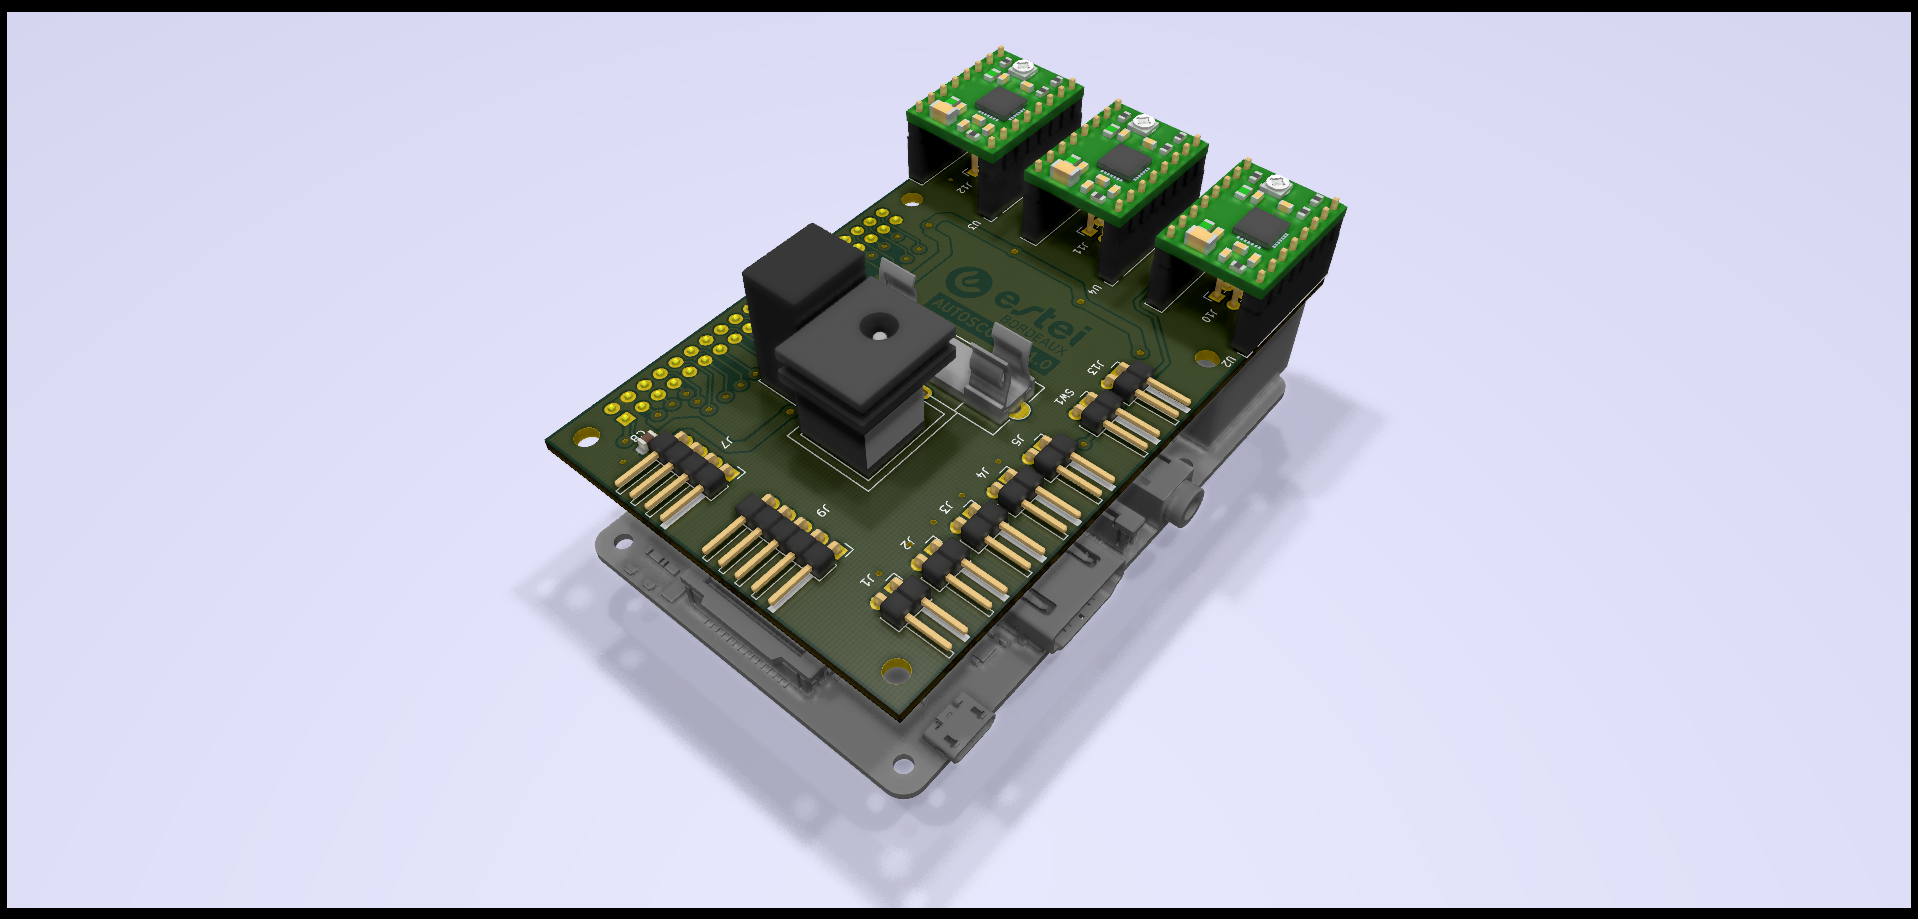
\includegraphics[width=1\linewidth]{\figures/kicad_3d_3.png}
    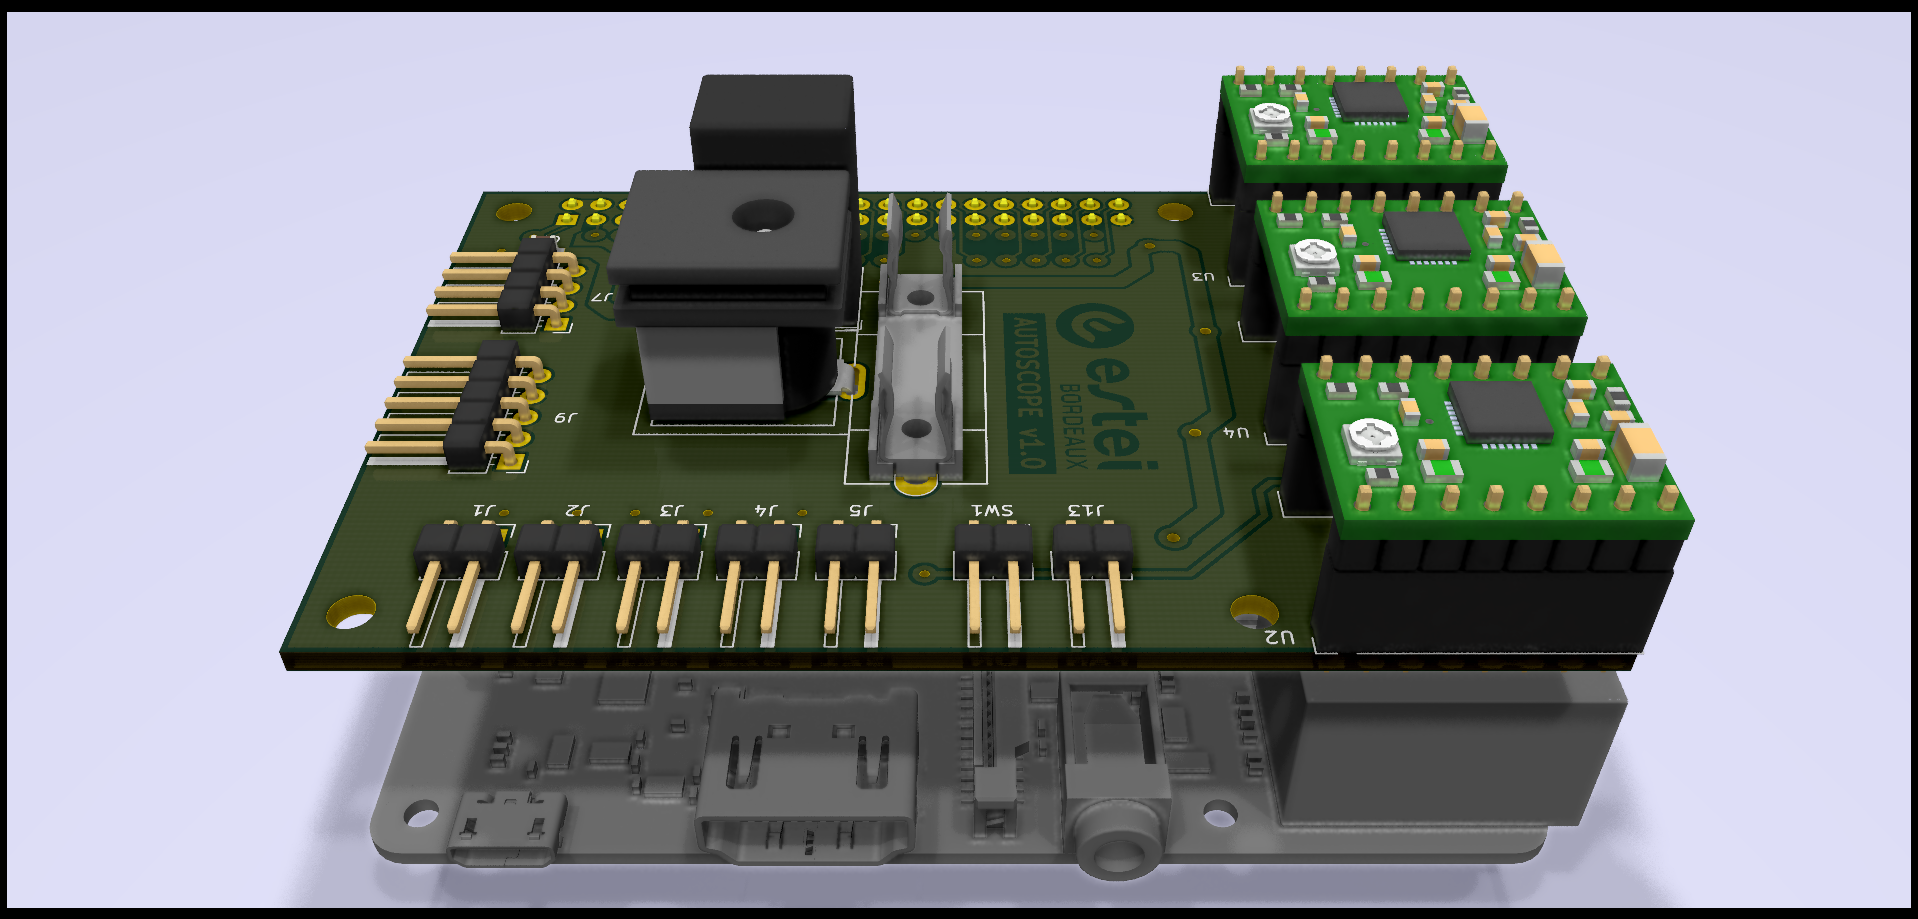
\includegraphics[width=0.495\linewidth]{\figures/kicad_3d_2.png}
    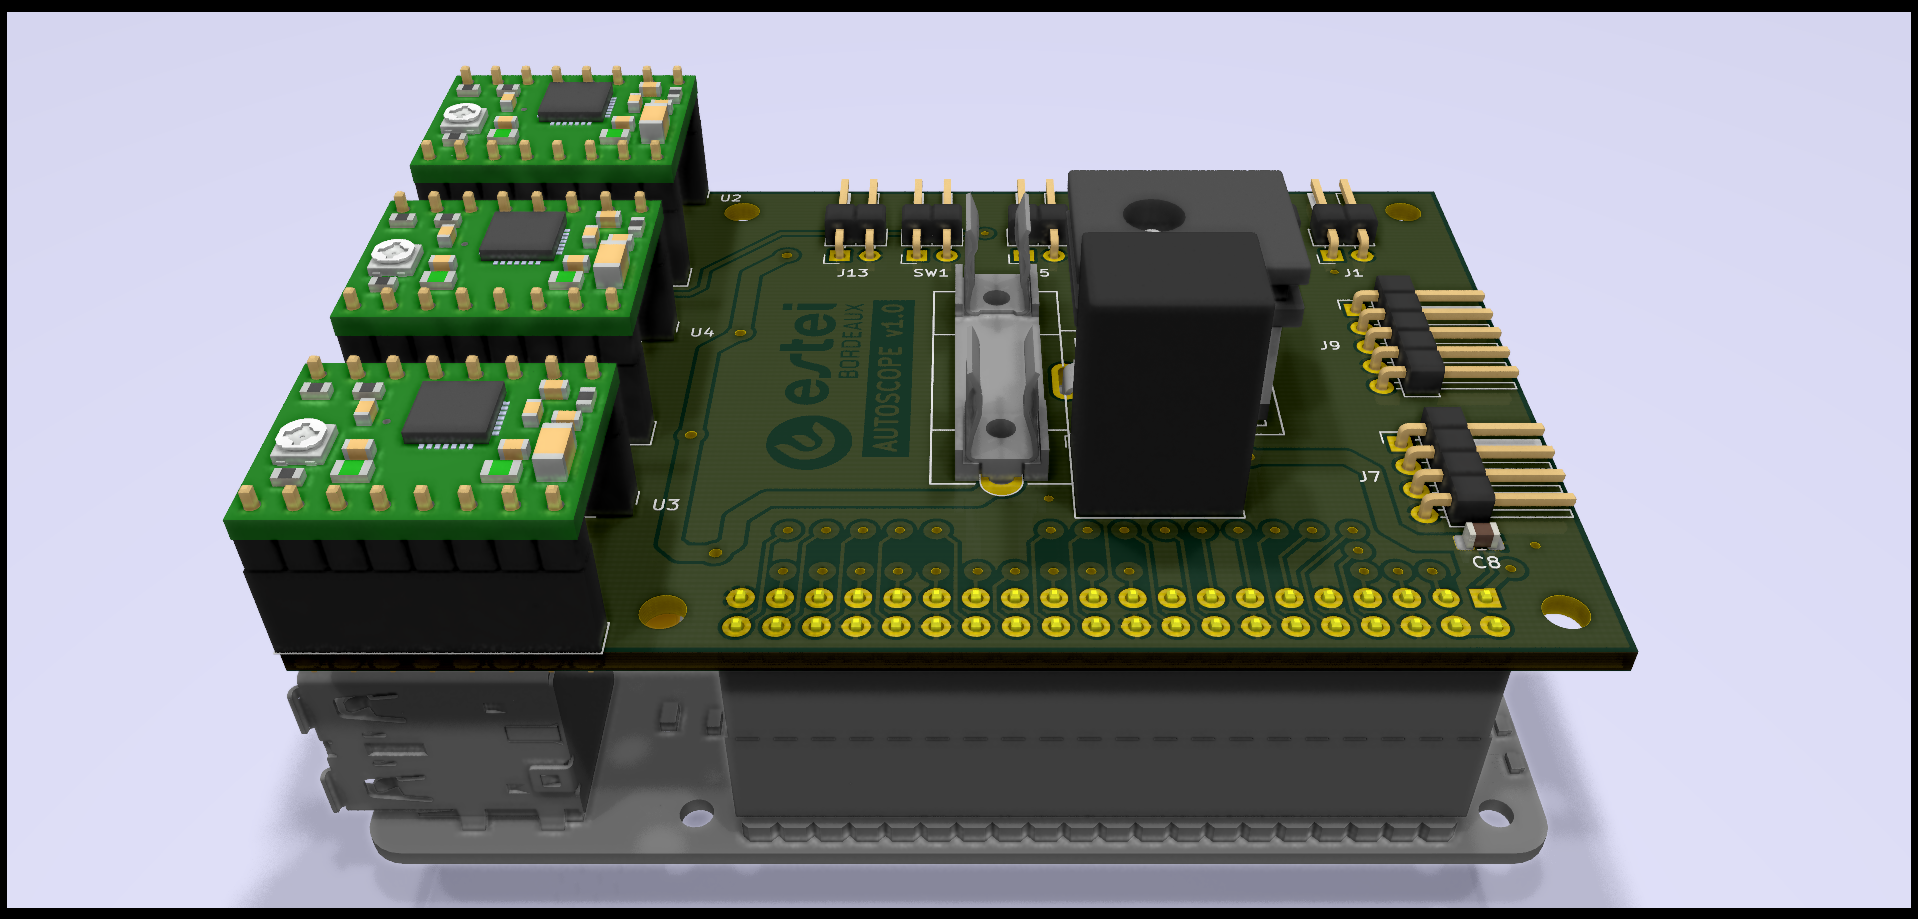
\includegraphics[width=0.495\linewidth]{\figures/kicad_3d_1.png}
    \decoRule
    \caption[
    Modélisation 3D de la carte pluggée sur la Raspberry-Pi]{
    Modélisation 3D de la carte pluggée sur la Raspberry-Pi}
    \label{fig:Modélisation 3D de la carte pluggée sur la Raspberry-Pi}
    \end{figure}

\vspace{1cm}

Au delà de l'aspect esthétique, la modélisation 3D permet d'avoir un aperçu du produit fini et de valider ou non le respect de certaines contraintes de design. Ou encore de repérer des vices que l'on ne voit pas forcément lors de la réalisation du typon, voire du schéma.

%\vspace{1cm}
\subsection{Allure générale de la carte}

Ainsi l'on observe d'abord l'allure générale de la carte~:

\begin{figure}[H]
    \centering
    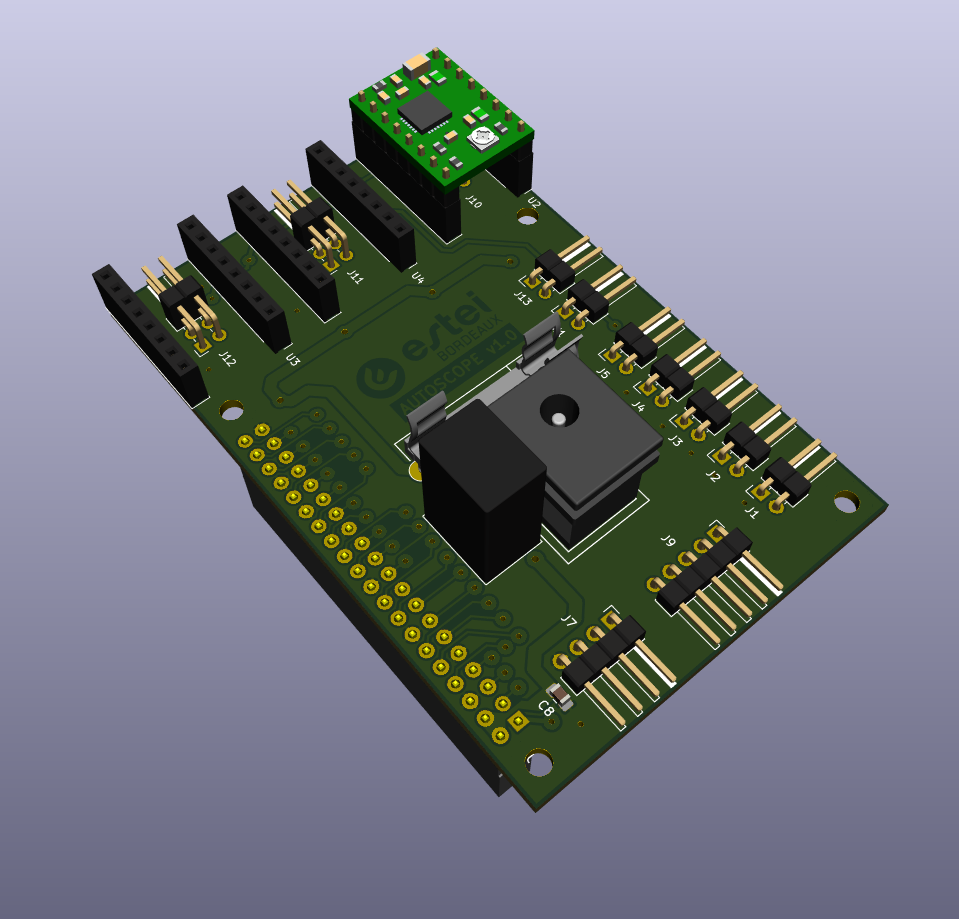
\includegraphics[width=0.49\linewidth]{\figures/kicad_3d_11_2.png}
    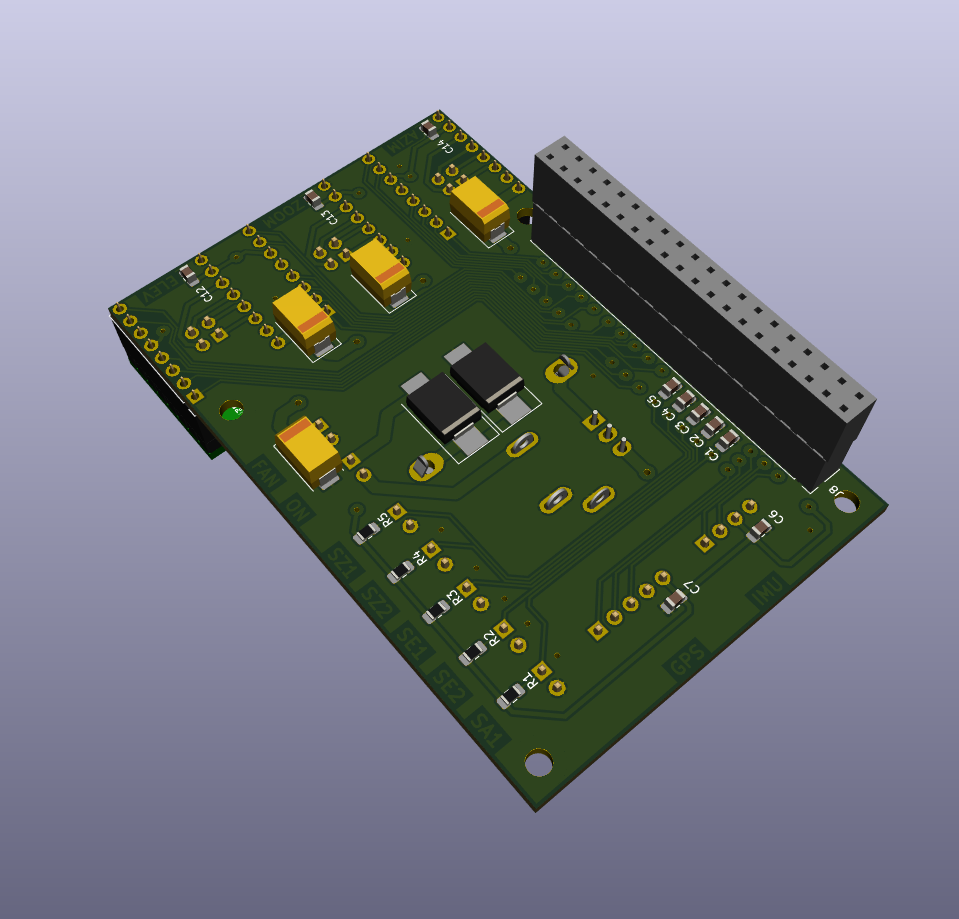
\includegraphics[width=0.49\linewidth]{\figures/kicad_3d_12_2.png}
    \decoRule
    \caption[
    Modélisation 3D de la carte avec et sans modules de contrôle moteur]{
    Modélisation 3D de la carte avec et sans modules de contrôle moteur}
    \label{fig:Modélisation 3D de la carte avec et sans modules de contrôle moteur}
    \end{figure}

%\vspace{1cm}
\subsection{Connecteurs des moteurs}

Ensuite l'on peut s'assurer de la pertinence de disposer les connecteurs des moteurs sous leurs contrôleurs~:

\begin{figure}[H]
    \centering
    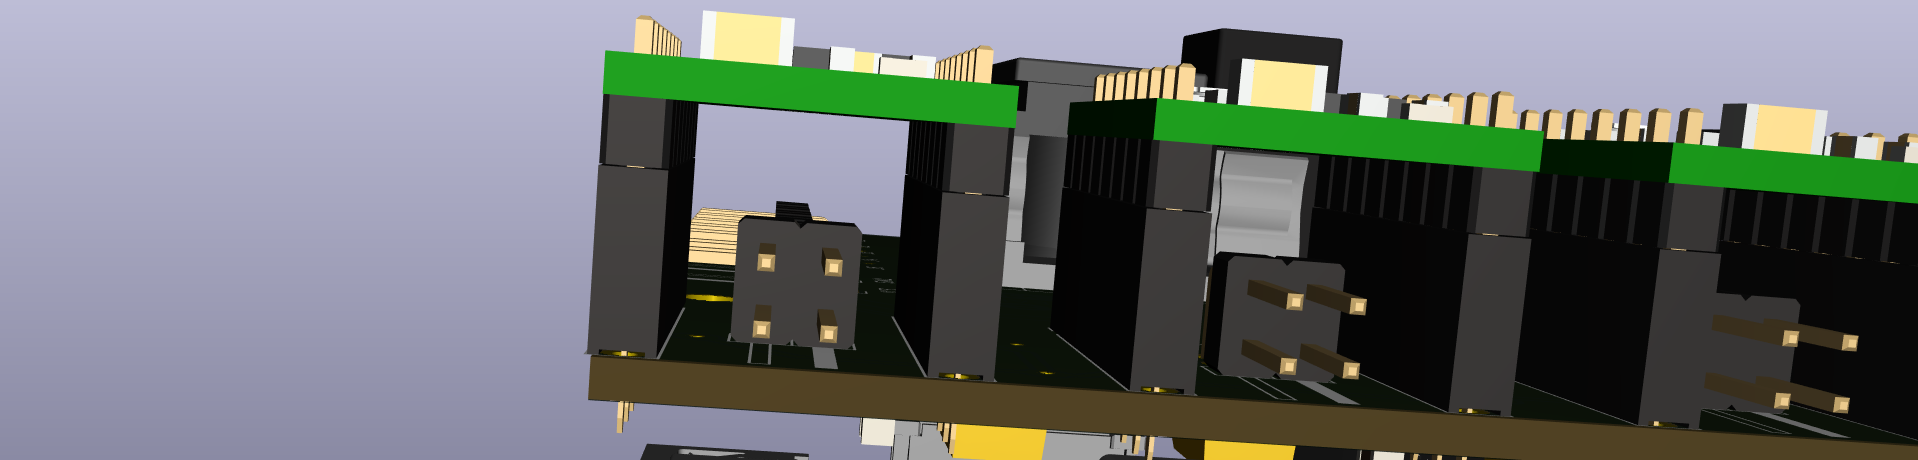
\includegraphics[width=1\linewidth]{\figures/kicad_3d_5_2.png}
    \decoRule
    \caption[
    Modélisation 3D de la carte~: zoom sur les connecteurs moteurs]{
    Modélisation 3D de la carte~: zoom sur les connecteurs moteurs}
    \label{fig:Modélisation 3D de la carte : zoom sur les connecteurs moteurs}
    \end{figure}

%\vspace{1cm}
\subsection{Emboîtement des cartes}

Puis on peut vérifier le correct emboîtement des cartes pour un espace les séparant de $19mm$, la longueur des entretoises utilisées. En particulier au niveau des condensateurs les plus volumineux~:

\begin{figure}[H]
    \centering
    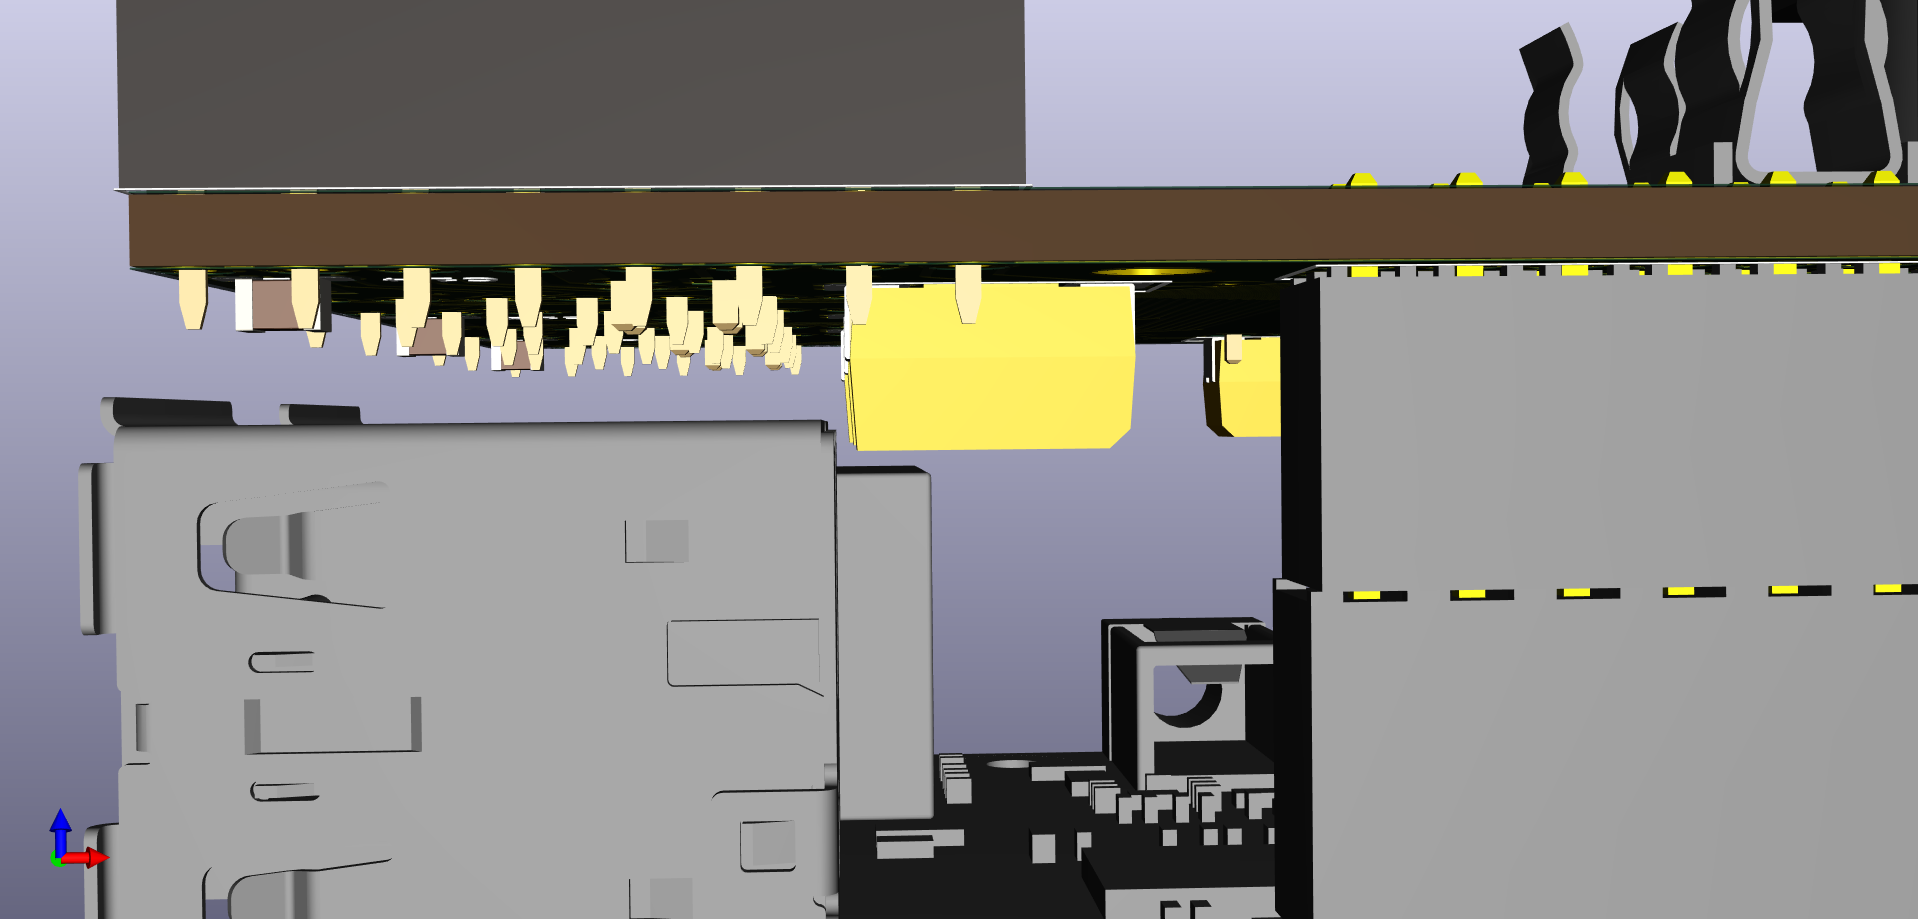
\includegraphics[width=0.49\linewidth]{\figures/kicad_3d_7_.png}
    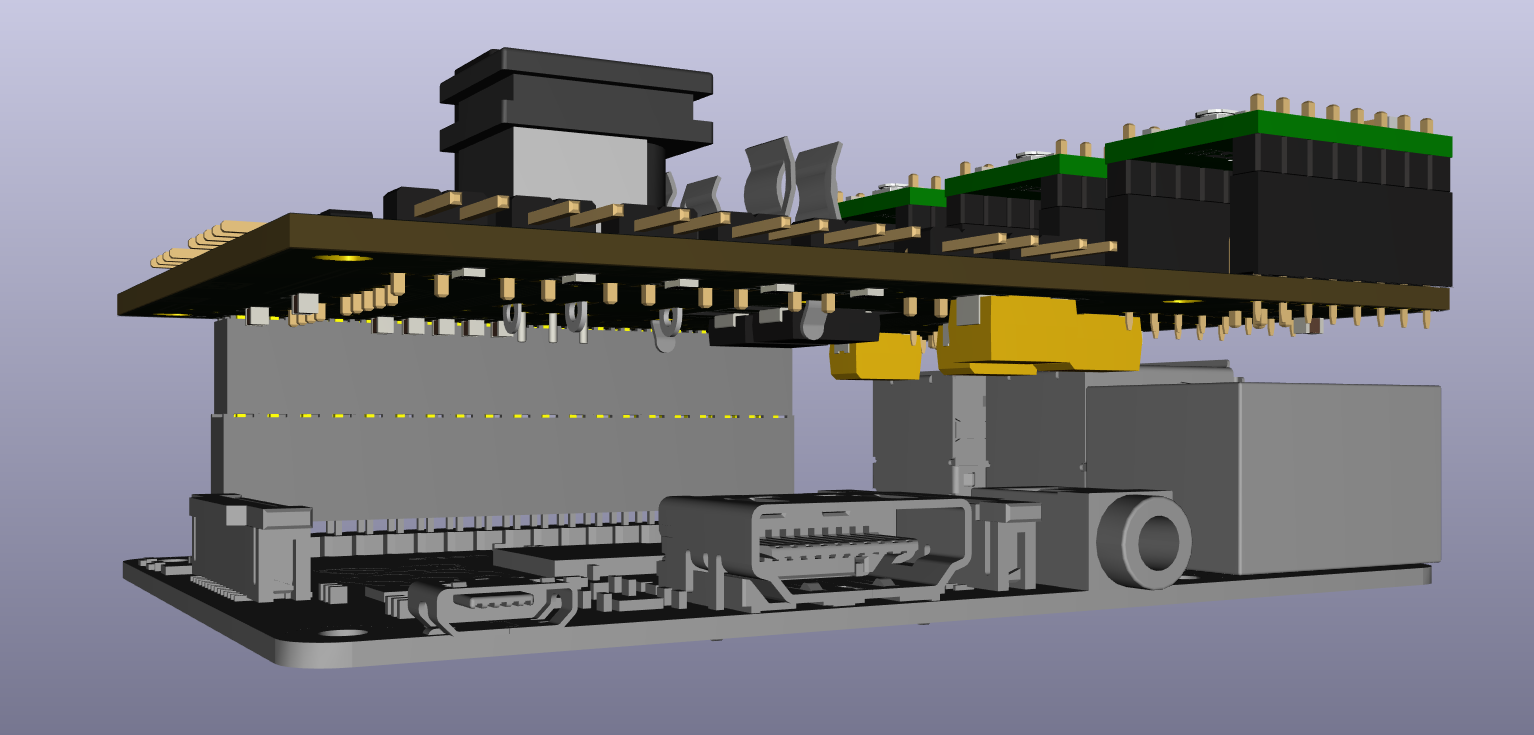
\includegraphics[width=0.49\linewidth]{\figures/kicad_3d_13_2.png}
    \decoRule
    \caption[
    Modélisation 3D de la carte~: zoom sur l'emboîtement des cartes]{
    Modélisation 3D de la carte~: zoom sur l'emboîtement des cartes}
    \label{fig:Modélisation 3D de la carte : zoom sur l'emboîtement des cartes}
    \end{figure}

%\vspace{1cm}
\subsection{Repères des connecteurs}

Enfin, question de commodité, des repères ont étés ajoutés pour indiquer le rôle de chaque connecteur. Ceux-ci se trouvent au niveau du connecteur associé, sur la face opposée du PCB, c'est-à-dire, sur la face coté Raspberry-Pi.

Placées sur le télescope, la Raspberry-Pi étant vouée à être sur le dessus, les repères sont sensés êtres visibles par l'utilisateur.

\begin{figure}[H]
    \centering
    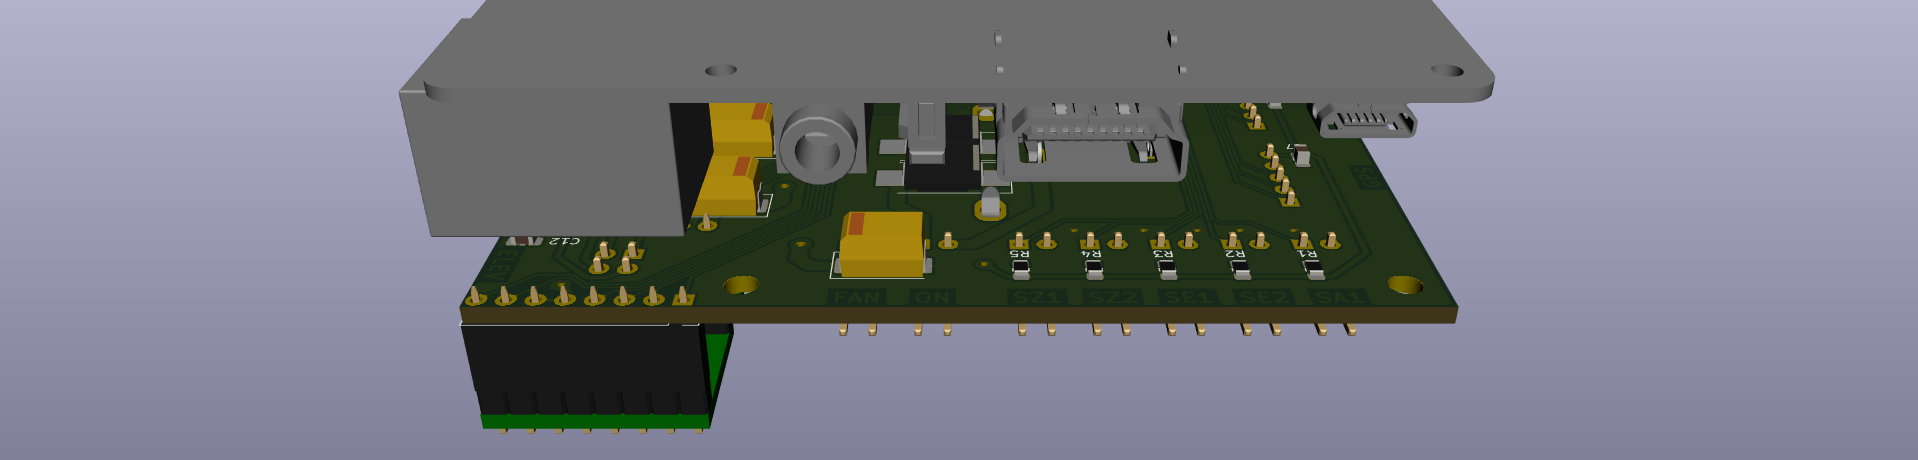
\includegraphics[width=1\linewidth]{\figures/kicad_3d_9_2.png}
    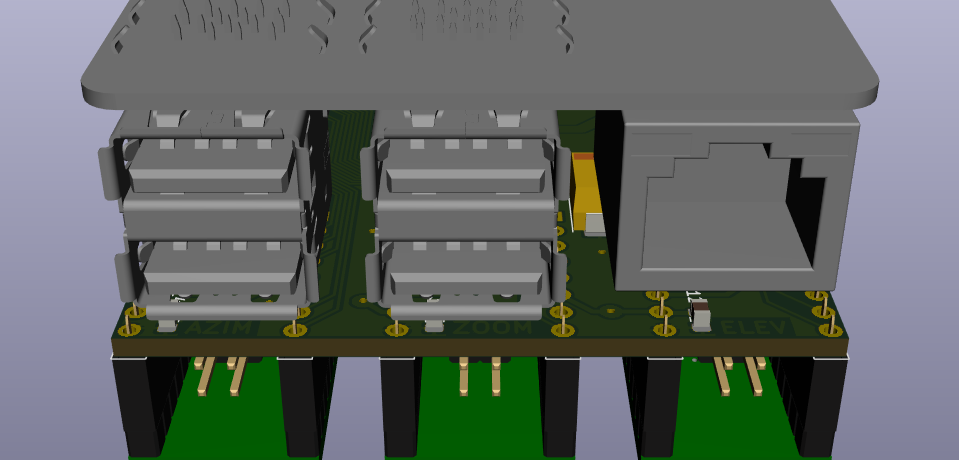
\includegraphics[width=0.495\linewidth]{\figures/kicad_3d_8_2.png}
    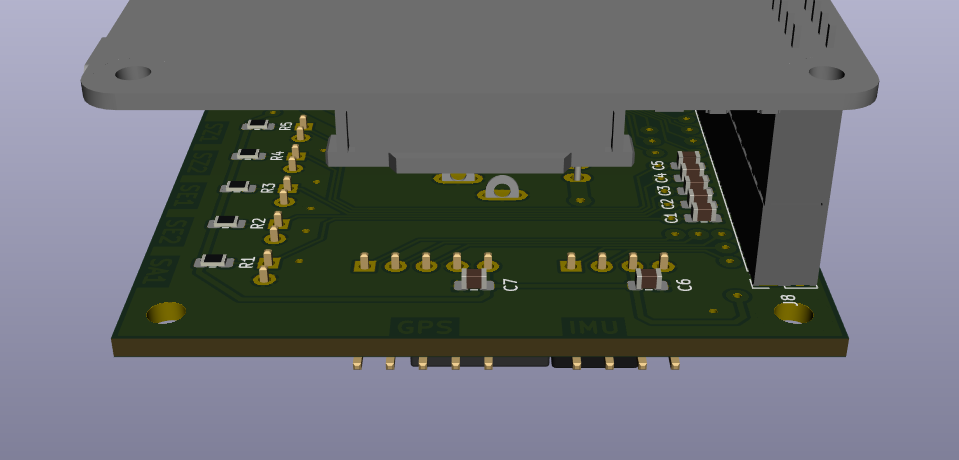
\includegraphics[width=0.495\linewidth]{\figures/kicad_3d_10_2.png}
    \decoRule
    \caption[
    Modélisation 3D de la carte~: zoom sur les repères des connecteurs]{
    Modélisation 3D de la carte~: zoom sur les repères des connecteurs}
    \label{fig:Modélisation 3D de la carte : zoom sur les repères des connecteurs}
    \end{figure}

\vspace{1cm}

\begin{itemize}[label=$\bullet$]
	\item AZIM~: Connecteur du moteur d'azimut.
	\item ZOOM~: Connecteur du moteur de zoom.
	\item ELEV~: Connecteur du moteur d'élévation.
	\item FAN~: Connecteur d'alimentation du ventilateur de refroidissement du miroir primaire.
	\item ON~: Connecteur d'un interrupteur On/Off d'alimentation du télescope.
	\item SZ1~: Connecteur du premier interrupteur de butée du moteur de zoom.
	\item SZ2~: Connecteur du second interrupteur de butée du moteur de zoom.
	\item SE1~: Connecteur du premier interrupteur de butée du moteur d'élévation.
	\item SE2~: Connecteur du second interrupteur de butée du moteur d'élévation.
	\item SA1~: Connecteur de l'unique interrupteur du moteur d'azimut.
	\item GPS~: Connecteur du module GPS.
	\item IMU~: Connecteur du module IMU (centrale inertielle).
	\end{itemize}

\subsection{Intégration du modèle 3D au télescope}

Il est possible d'exporter le modèle 3D des deux cartes emboîtées et ainsi de l'utiliser comme élément lors de la modélisation du télescope. Ci-dessous un aperçu des cartes grossièrement placées sur le modèle du télescope~:

\begin{figure}[H]
    \centering
    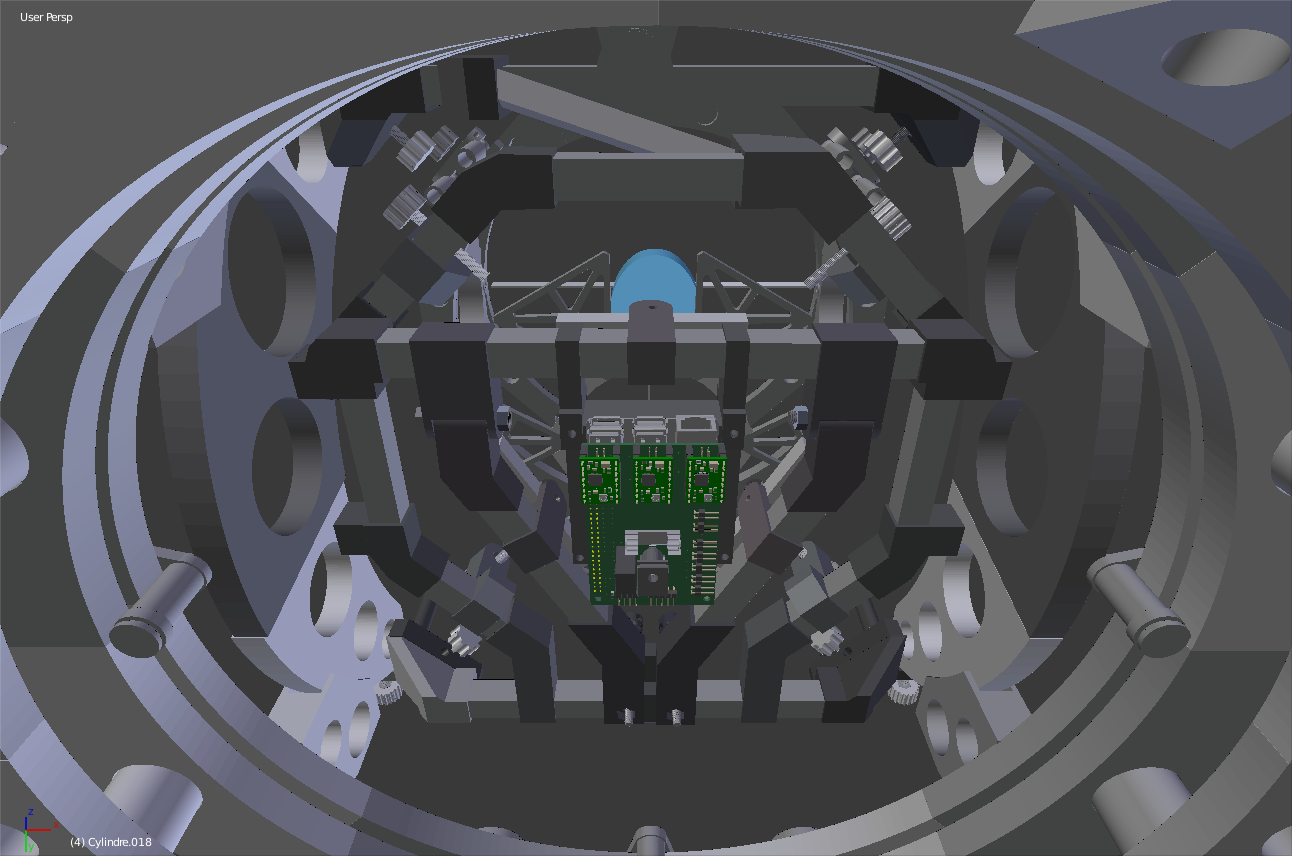
\includegraphics[width=0.495\linewidth]{\figures/blender_1.png}
    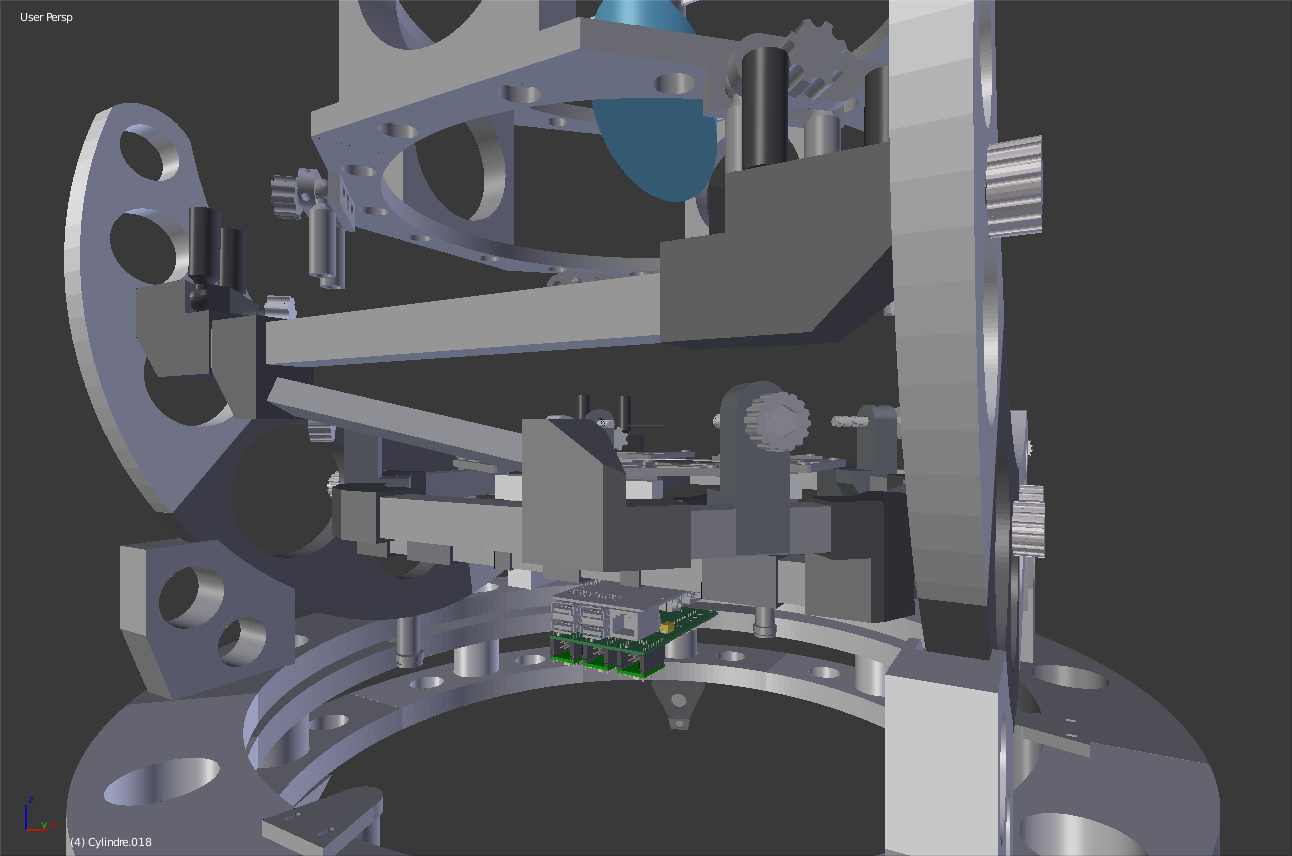
\includegraphics[width=0.495\linewidth]{\figures/blender_2.png}
    \decoRule
    \caption[
    Modélisation 3D du télescope grossièrement équipé de ses cartes électroniques]{
    Modélisation 3D du télescope grossièrement équipé de ses cartes électroniques}
    \label{fig:Modélisation 3D du télescope grossièrement équipé de ses cartes électroniques}
    \end{figure}

\section{Fabrication et connectique}

La fabrication de la carte ne présente pas de subtilité particulière. Il est toutefois conseillé d'être méthodique quant à l'ordre de soudure des composants pour ne pas être gêné par certains en en soudant d'autres.

Aussi il est conseillé de placer les contrôleurs moteur sur leurs connecteurs support (U2, U3 et U4) pour souder lesdits support à la carte. Cela pour que les connecteurs supports restent parallèles et qu'emboîter le contrôleur ne pose pas de problème.

\begin{figure}[H]
    \centering
	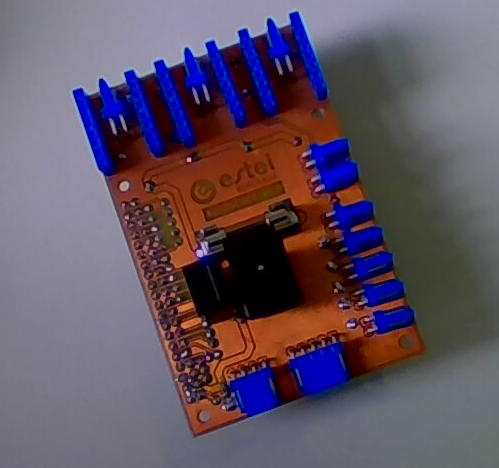
\includegraphics[width=0.32\linewidth]{\figures/photo_hardware1.png}
	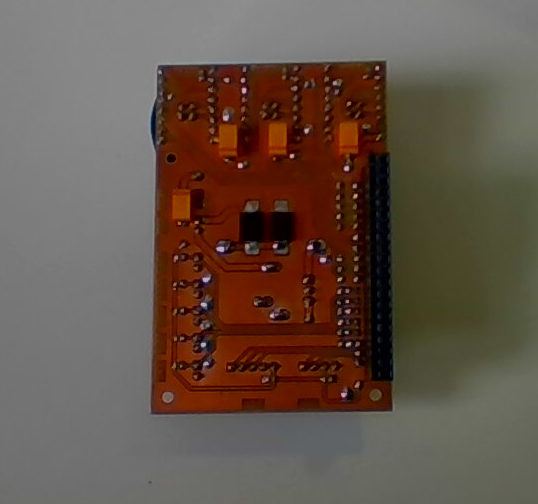
\includegraphics[width=0.32\linewidth]{\figures/photo_hardware3.png}
	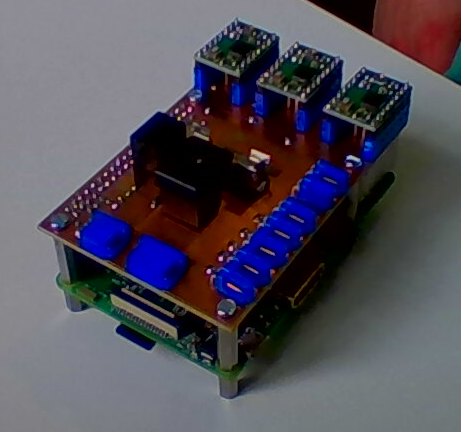
\includegraphics[width=0.32\linewidth]{\figures/photo_hardware2.png}
    \decoRule
    \caption[
    Photos de la carte seule et pluggée sur la Raspberry-Pi]{
    Photos de la carte seule et pluggée sur la Raspberry-Pi}
    \label{fig:Photos de la carte seule et pluggée sur la Raspberry-Pi}
	\end{figure}

\vspace{1cm}

Quant au raccordement des différents périphériques, celui-ci devra être fait une fois la structure du télescope montée, ou du moins une fois le modèle 3D de la structure dans sa version définitive.

\begin{figure}[H]
    \centering
	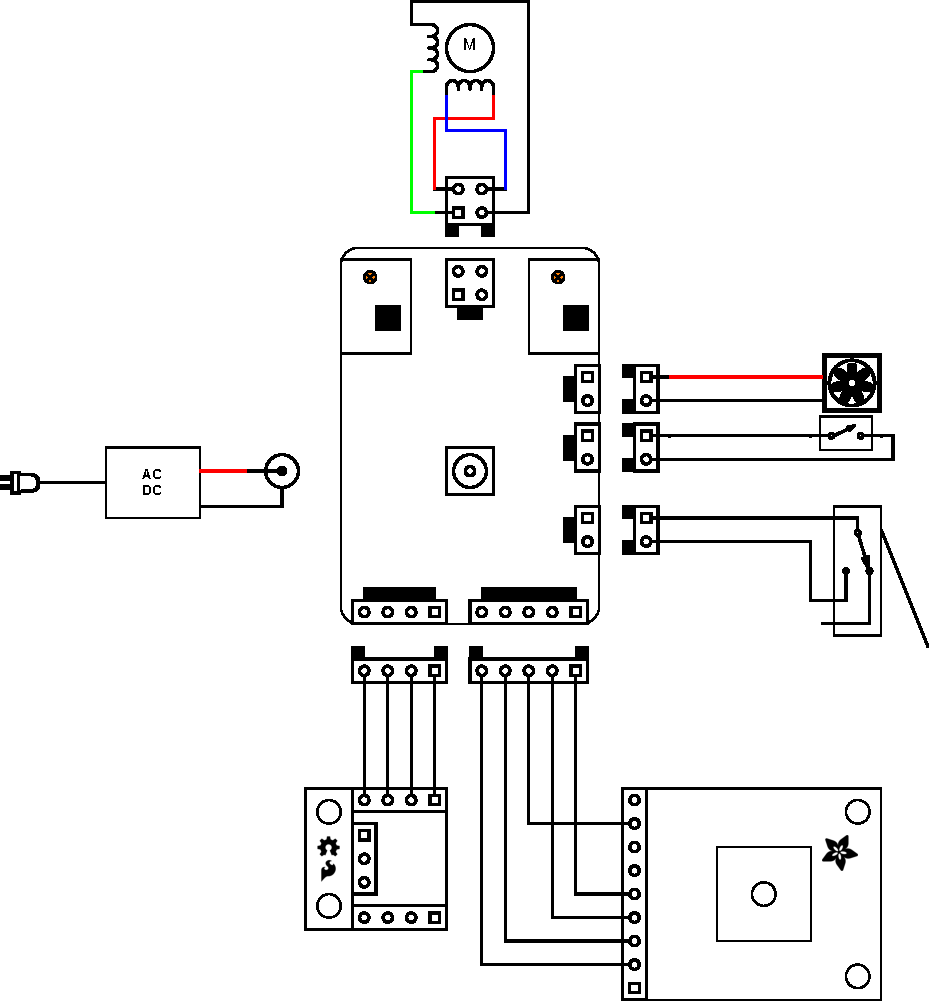
\includegraphics[width=0.9\linewidth]{\figures/sch_connection.pdf}
    \decoRule
    \caption[
    Schéma de raccordement des périphériques de la carte]{
    Schéma de raccordement des périphériques de la carte}
    \label{fig:Schéma de raccordement des périphériques de la carte}
	\end{figure}


\vspace{1cm}

Remarque~: Compte tenu de la proximité du connecteur de l'interrupteur \codeinline{text}{On/Off} et du connecteur d'alimentation $+12V$ du ventilateur, il est impératif d'être vigilent à ne pas brancher l'interrupteur à la mauvaise place sous peine de faire fondre le fusible ou pire, d'endommager la carte.

\vspace{1cm}

Remarque~: On remarque un routage maladroit puisque la nappe jusqu'au GPS doit être croisée.

\section{Validation}

\subsection{Tests de continuité et de fuite de courant}

Ces test, bien qu'élémentaires, permettent de valider la fonctionnement de la quasi-intégralité de la carte. Une relecture attentive du schéma de la carte, en particulier du câblage des connecteurs est impérative.

\vspace{1cm}

Il s'agit de vérifier pour chaque broche du connecteur $40$ broches que le courant se propage correctement jusqu'à la broche correspondante d'un autre connecteur, à l'autre extrémité de la piste. Vérifier également qu'aucune fuite de courant ou court-circuit n'existe vers les pistes voisines ou la masse.

\subsection{Test de l'environnement des interrupteurs de butée}

Pour valider le fonctionnement des boutons, on alimente la carte et on mesure la tension de sortie à l'état enfoncé et relâché de chaque bouton~:

\begin{figure}[H]
    \centering
    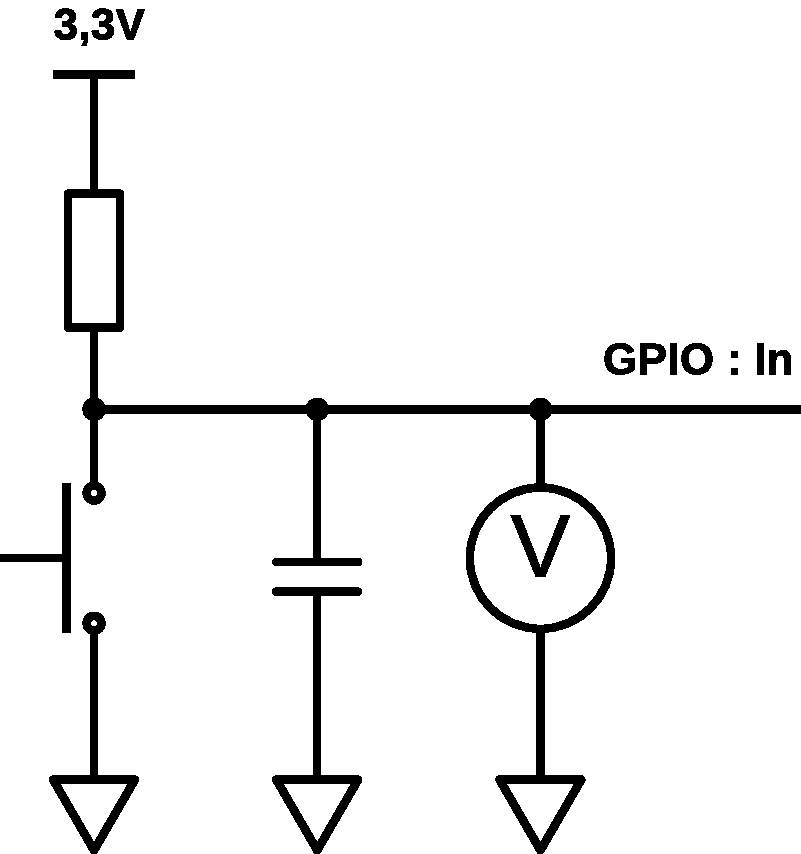
\includegraphics[width=0.3\linewidth]{sch_test_button.pdf}
    \decoRule
    \caption[
    Procédure de test de l'environnement des boutons]{
    Procédure de test de l'environnement des boutons}
    \label{fig:Procédure de test de l'environnement des boutons}
	\end{figure}

\begin{figure}[H]
    \centering
	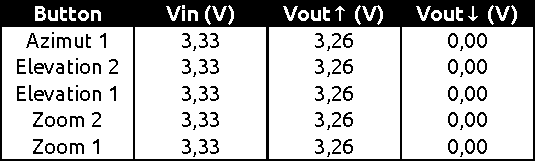
\includegraphics[width=0.5\linewidth]{tab_test_button.pdf}
    \decoRule
    \caption[
    Mesure de la tension de sortie des boutons]{
    Mesure de la tension de sortie des boutons}
    \label{fig:Mesure de la tension de sortie des boutons}
	\end{figure}

%\vspace{1cm}

\begin{figure}[H]
    \centering
	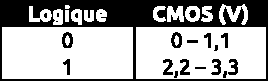
\includegraphics[width=0.25\linewidth]{tab_cmos.pdf}
    \decoRule
    \caption[
    Niveaux de tensions de la logique CMOS]{
    Niveaux de tensions de la logique CMOS}
    \label{fig:Niveaux de tensions de la logique CMOS}
	\end{figure}

\vspace{1cm}

Les niveaux électriques haut et bas sont largement inclus dans les plages de tolérances CMOS, les boutons sont fonctionnels.

\subsection{Test de l'alimentation} %TODO test TVS

Pour tester l'alimentation, on vérifie d'abord le fonctionnement du convertisseur DC/DC $12V/5V$ par le montage suivant~:

\begin{figure}[H]
    \centering
    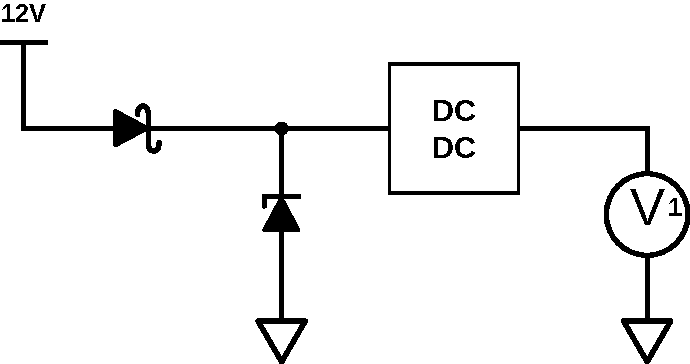
\includegraphics[width=0.5\linewidth]{sch_test_dcdc.pdf}
    \decoRule
    \caption[
    Procédure de test du convertisseur DC/DC]{
    Procédure de test du convertisseur DC/DC}
    \label{fig:Procédure de test du convertisseur DC/DC}
	\end{figure}

\vspace{1cm}

Pour une tension d'entrée $V_{in}=12,10V$, l'on a une tension de sortie $V_{1}=5,02V$. Le convertisseur fonctionne.

\vspace{1cm}

Ensuite, pour tester le système de protection aux surtensions, on ajoute une résistance pour limiter le courant et on augmente la tension d'alimentation. Cette protection est destinée aux condensateurs de découplage de l'alimentation de puissance dont la tension de claquage est de $16V$. Le convertisseur DC/DC et les contrôleurs moteur pouvant tolérer respectivement $32V$ et $35V$ et les moteurs étant généralement moins sensibles aux surtensions.

\begin{figure}[H]
    \centering
    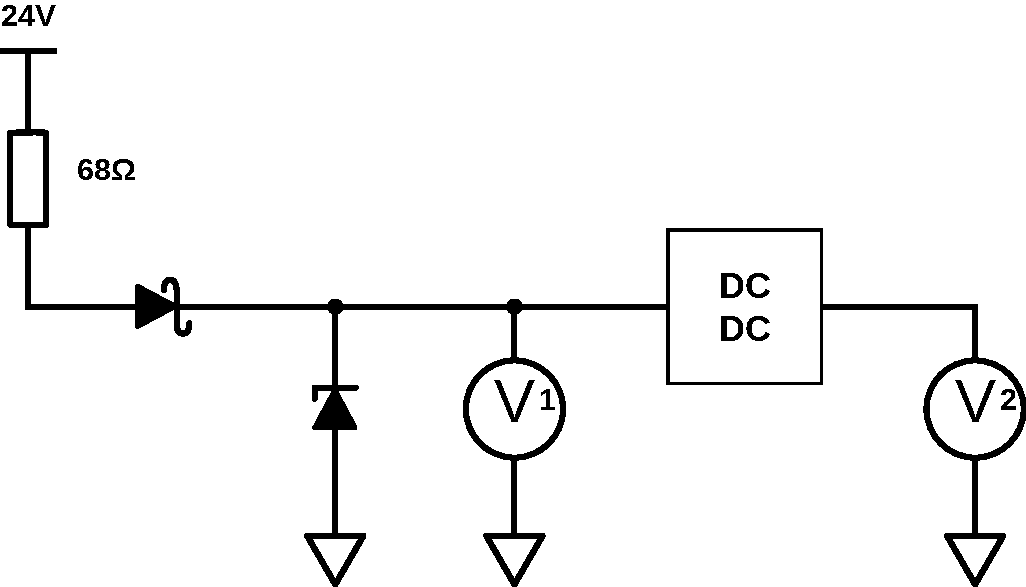
\includegraphics[width=0.6\linewidth]{sch_test_tvs.pdf}
    \decoRule
    \caption[
    Procédure de test de la protection aux surtensions]{
    Procédure de test de la protection aux surtensions}
    \label{fig:Procédure de test de la protection aux surtensions}
	\end{figure}

\vspace{1cm}

Pour une tension d'entrée $V_{in}=23,3V$, l'on a des tensions $V{1}=V$ et $V_{2}=5,03V$. La diode adaptée à une tension de $12V$ a une tension de coupure comprise entre $13,3V$ et $14,7V$ pour un courant de $1mA$. La protection fonctionne comme elle le devrait, la tension n'excédant pas $16V$. 

\vspace{1cm}

Concernant le connecteur d'alimentation, la solution semble bonne puisque la carte est capable de pivoter aisément autour du câble d'alimentation sans que celui-ci ne se décroche.

